% Provenance (never printed): old seconde/premiere S material on the water
% cycle on land (the drainage basin, river discharge, floods and their
% management); see sources/book2/PROVENANCE.md. The Varden basin is computed
% in figdata/grade-10/varden_basin.py from figdata/shared/region.py; the
% Potomac record in figdata/grade-10/flood_frequency.py.
\chapter{流域、河流与洪水}\label{ch:g10:drainage-basins}

一条河可能在雨停两天后才涨水，而它所在的城镇
根本没有下过雨。淹没街道的水，其实早在上游很远的山丘上落下；
它沿山坡流入溪涧，溪涧汇入
它所在的河流，一并涌向城镇。要理解一次洪水，
必须跳出河流本身，看清供给它的整片区域，
并追踪水在其中的运动。本章将定义这一区域——\omterm{def:g10:drainage-basins:drainage-basin}{流域}；
测量河流所携带的水量——\omterm{def:g10:drainage-basins:discharge}{流量}；追踪洪水经过河流某一点时的变化过程；
并说明如何利用长期的洪水记录，
判断某一特定洪水多久会重现一次。

\begin{omfigure}
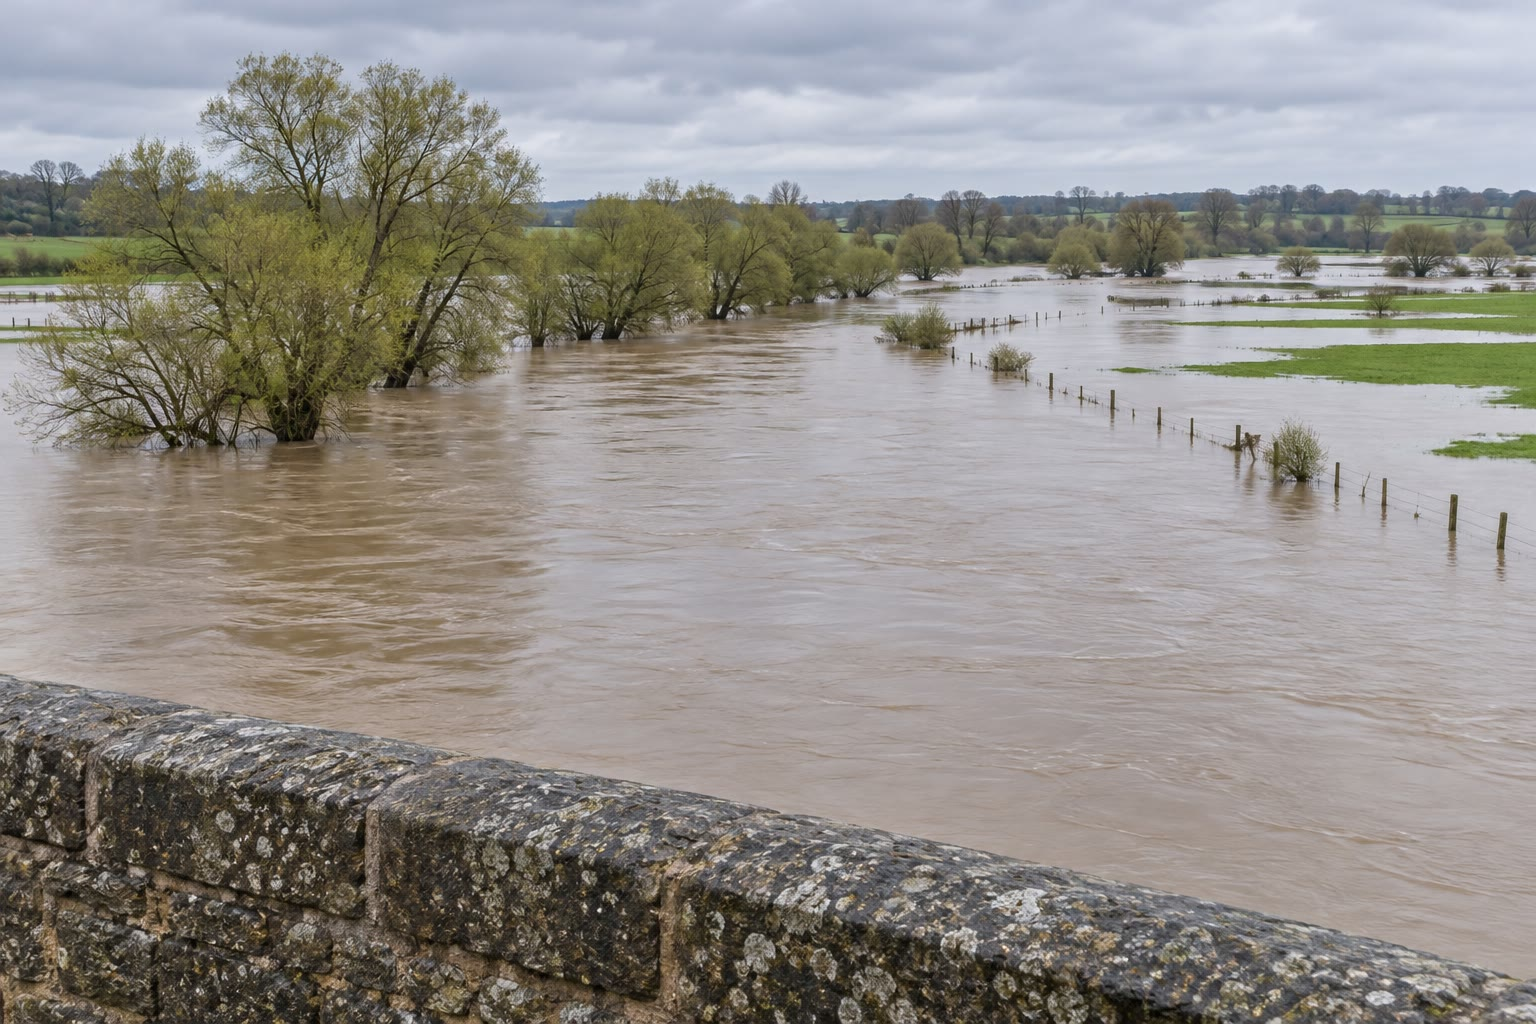
\includegraphics[width=0.8\linewidth]{images/book2/ai/g10-river-flood-meadows.jpg}

{\small 从石桥上看到的洪水中的河流：棕色的河水裹挟着泥沙，
已漫出河道，淹没了河漫滩上的草地，
直至围栏和平时沿河岸生长的树木。}
\end{omfigure}

\begin{recall}
落到地面的雨水，或渗入地下，或沿地表流走，或
蒸发；水循环将其带回海洋（见物理教材）。水渗入透水的岩石，充满地下水位以下的岩层，
形成含水层，为泉和河流提供水源（见第 1 册，
六年级）。河流在平坦的河漫滩上蜿蜒成曲流，
洪水时淹没河漫滩（见第 1 册，五年级）。等高线连接高度相同的点；
瓦尔登丘陵是本系列地图上所绘的地区（见第 1 册，
二年级和九年级）。
\end{recall}

\begin{safety}
洪水的水远比看上去危险。约 \qty{15}{cm} 深、流速较快的水
就能把成年人冲倒；约 \qty{30}{cm} 深的水便能卷走一辆汽车，
而水下的道路可能已经塌陷。切勿步行或驾车进入洪水：
请掉头，改走其他路线。
% ledger: nws:flood-water
\end{safety}

\section{流域}

每一滴不被蒸发、也不深入渗透的雨水，都会顺坡向低处流去。
它沿地面最陡的坡向流动，先汇入细沟，再汇入溪流，
溪流汇成河流。所有水最终流入同一条河流的土地，
构成一个整体。

\begin{definition}[流域；分水岭]\label{def:g10:drainage-basins:drainage-basin}
河流上某一点的\emph{流域}\index{流域}，是
这样一片陆地的全部范围：其径流流向该点上游的河流，
并流经该点。\emph{分水岭}\index{分水岭}是分隔两个相邻流域的界线：它
沿着地表的山脊延伸，落在界线两侧的雨水，
流入不同的河流。
%
\end{definition}

任一\omterm{def:g10:drainage-basins:drainage-basin}{流域}都是针对河流上的某一点定义的，该点即其\emph{出口}：
河流入海处的\omterm{def:g10:drainage-basins:drainage-basin}{流域}最大，而其上游每一点
的\omterm{def:g10:drainage-basins:drainage-basin}{流域}都较小，且包含于其内。两滴相距 1 米、落在
\omterm{def:g10:drainage-basins:drainage-basin}{分水岭}两侧，可能流入不同的河流，甚至
流入不同的海洋。

\subsection*{瓦尔登河的流域}

借助计算机，由高程图只需几步即可求出\omterm{def:g10:drainage-basins:drainage-basin}{流域}。
地图被切分成小方格，此处每格边长为 \qty{50}{m}。对每一个方格，
计算机考察其八个相邻方格，并将水送往
坡度最陡的低处方格。（若某个小洼地没有更低的相邻方格，
则先将其填平至溢出的高度，如同水坑被填满一样。）依此逐格推进，
便可追踪地图上任一点雨滴的路径。
凡雨滴能到达河流的方格，
便构成\omterm{def:g10:drainage-basins:drainage-basin}{流域}。

\begin{omfigure}
\begin{tikzpicture}
\begin{axis}[axis equal image, xmin=0, xmax=10, ymin=0, ymax=8, width=0.86\linewidth,
  tick label style={font=\scriptsize}, xlabel={东 (km)}, ylabel={北 (km)},
  label style={font=\small}, enlargelimits=false]
\addplot[fill=omDef!14, draw=none, even odd rule] table {figdata/out/grade-10-varden_basin-fill.dat};
\addplot[contour, line width=0.25pt, opacity=0.7] table {figdata/out/shared-region-contours.dat};
\addplot[index contour, opacity=0.8] table {figdata/out/shared-region-index-contours.dat};
\addplot[river, line width=1.6pt] table {figdata/out/shared-region-river.dat};
\addplot[omThm, line width=1.4pt, dashed] table {figdata/out/grade-10-varden_basin-divide.dat};
\addplot[omWxRain, line width=0.9pt, -{Stealth[length=5pt]}] table {figdata/out/grade-10-varden_basin-path1.dat};
\addplot[omWxRain, line width=0.9pt, -{Stealth[length=5pt]}] table {figdata/out/grade-10-varden_basin-path2.dat};
\addplot[omWxRain, line width=0.9pt, -{Stealth[length=5pt]}] table {figdata/out/grade-10-varden_basin-path3.dat};
\addplot[omWxRain, line width=0.9pt, -{Stealth[length=5pt]}] table {figdata/out/grade-10-varden_basin-path4.dat};
\fill[omWxRain] (axis cs:2,7.4) circle (2.2pt);
\fill[omWxRain] (axis cs:4,1.8) circle (2.2pt);
\fill[omWxRain] (axis cs:8.6,6.6) circle (2.2pt);
\fill[omWxRain] (axis cs:2.5,0.7) circle (2.2pt);
\node[font=\footnotesize, fill=white, fill opacity=0.85, text opacity=1, inner sep=1.5pt, text=omThm] at (axis cs:6.0,6.75) {分水岭};
\node[font=\footnotesize, fill=white, fill opacity=0.85, text opacity=1, inner sep=1.5pt, text=omThm] at (axis cs:3.5,1.1) {分水岭};
\node[font=\footnotesize, fill=white, fill opacity=0.85, text opacity=1, inner sep=1.5pt, align=center] at (axis cs:5.3,7.55) {流域外：\\水向北流走};
\node[font=\footnotesize, fill=white, fill opacity=0.85, text opacity=1, inner sep=1.5pt, align=right, anchor=east] at (axis cs:9.85,3.35) {出口};
\draw[-{Stealth[length=6pt]}, line width=1pt, omRiver] (axis cs:9.3,3.7) -- (axis cs:9.95,4.15);
\node[font=\footnotesize, fill=white, fill opacity=0.85, text opacity=1, inner sep=1.5pt] at (axis cs:1.1,4.75) {河流};
\end{axis}
\end{tikzpicture}

{\small 瓦尔登丘陵地图上瓦尔登河的\omterm{def:g10:drainage-basins:drainage-basin}{流域}（阴影部分），
由计算每个边长为
\qty{50}{m} 方格的水沿最陡坡向流下而得出；等高线间距为 \qty{50}{m}。虚线为
\omterm{def:g10:drainage-basins:drainage-basin}{分水岭}；蓝线为四滴雨滴（圆点）的路径。
其中两滴到达河流，向东流至出口，
即河流离开地图之处；另外两滴落在\omterm{def:g10:drainage-basins:drainage-basin}{分水岭}之外，
离开地图，流向其他河流。}
\end{omfigure}

\omterm{def:g10:drainage-basins:drainage-basin}{流域}覆盖地图总面积 \qty{80}{km^2} 中的 \qty{66}{km^2}，约占
其五分之四。北部，\omterm{def:g10:drainage-basins:drainage-basin}{分水岭}沿丘陵的脊线延伸，
并经过其顶峰；越过顶峰后，地势背离河流倾斜，水流汇入另一山谷。
西南角还有一小片区域也排出图外。
河流从西侧进入地图，因此其完整\omterm{def:g10:drainage-basins:drainage-basin}{流域}更大，
它还包括上游的土地，这些土地位于
地图边缘之外。
% values computed in figdata/grade-10/varden_basin.py (basin_km2 66.19, map_km2 80)

\subsection*{最大的河流}

河流可以按\omterm{def:g10:drainage-basins:drainage-basin}{流域}面积和所携带的水量进行比较。
世界上最大的河流是亚马孙河，遥遥领先于其他河流。
密西西比河是美国最大的河流，\omterm{def:g10:drainage-basins:drainage-basin}{流域}面积约为 \num{1150000} 平方英里，
约 298 万 \unit{km^2}，\omterm{def:g10:drainage-basins:drainage-basin}{流域}范围涵盖美国和加拿大。
% ledger: kammerer:mississippi

\section{流量}

\begin{definition}[流量]\label{def:g10:drainage-basins:discharge}
河流在某点的\emph{流量}\index{流量}，是指
每秒钟流过河流某一截面的水的体积。
其单位为立方米每秒，\unit{m^3/s}。
\end{definition}

\omterm{def:g10:drainage-basins:discharge}{流量}为 \qty{1}{m^3/s}，即每秒一千升，
即每天 \qty{86400}{m^3}。水流在河道中部靠近水面处最快，
沿河床和河岸处最慢，因为那里的水与之摩擦；
\emph{平均速度}是指在整个
横截面上取平均的速度。

\begin{proposition}[流量、速度与截面]\label{prop:g10:drainage-basins:discharge}
河流的\omterm{def:g10:drainage-basins:discharge}{流量} $Q$ 等于水的平均速度 $v$
与过水截面面积 $A$ 的乘积：
\[
Q = v\,A.
\]
\end{proposition}

\begin{proof}
设在时间 $t$ 内，流经该截面的水向前移动了
距离 $v\,t$，于是充满了一段截面积为 $A$、长度为 $v\,t$ 的河段，
其体积为 $A\,v\,t$。以时间 $t$ 除以该体积，
即得每秒的体积 $Q = v\,A$。
\end{proof}

截面积为 \qty{50}{m^2}、平均速度为
\qty{1.2}{m/s} 的河流，其\omterm{def:g10:drainage-basins:discharge}{流量}为 $1.2 \times 50 = \qty{60}{m^3/s}$。发洪水时，两个因素都会增大：
水位加深、河面变宽，截面随之增大，
水流也更快。

\subsection*{流量的测量}

由于流速在河道各处不同，需要在多个
点进行测量。将河流划分为竖直的条带，在每个条带中测量水深和
流速，再将各条带的\omterm{def:g10:drainage-basins:discharge}{流量}相加。

\begin{method}[流速–面积法]\label{met:g10:drainage-basins:velocity-area}
\begin{enumerate}
  \item 在河面上拉开测量卷尺，
        沿其选取间距相等的 $w$ 的竖直测线。
  \item 在每条测线处，用流速仪测量水深 $d$，
        以及该水深范围内水的平均速度 $v$。
  \item 每条测线代表一个宽为 $w$、面积为 $w\,d$ 的条带，其
        \omterm{def:g10:drainage-basins:discharge}{流量}为 $v\,w\,d$。
  \item 将所有条带的\omterm{def:g10:drainage-basins:discharge}{流量}相加：$Q = \sum v\,w\,d$。
        截面积为 $A = \sum w\,d$，平均速度为 $Q/A$。
\end{enumerate}
\end{method}

\begin{omfigure}
\begin{tikzpicture}[x=0.9cm, y=1.6cm, font=\footnotesize]
  % water
  \fill[omSea] (0,0) -- (1,-0.4) -- (2,-0.75) -- (3,-1.0) -- (4,-1.25) -- (5,-1.4) -- (6,-1.3)
     -- (7,-1.1) -- (8,-0.8) -- (9,-0.5) -- (10,-0.2) -- (10.5,0) -- cycle;
  \fill[omDef!22] (4,0) -- (4,-1.25) -- (5,-1.4) -- (6,-1.3) -- (6,0) -- cycle;
  % bed
  \draw[line width=0.9pt, brown!60!black] (-0.6,0.35) -- (0,0) -- (1,-0.4) -- (2,-0.75) -- (3,-1.0) -- (4,-1.25)
     -- (5,-1.4) -- (6,-1.3) -- (7,-1.1) -- (8,-0.8) -- (9,-0.5) -- (10,-0.2) -- (10.5,0) -- (11.1,0.35);
  \draw[omDef!70!black, line width=0.5pt] (0,0) -- (10.5,0);
  % verticals
  \foreach \x/\d/\v/\dx in {1/0.4/0.3/0.3, 3/1.0/0.6/0, 5/1.4/0.8/0, 7/1.1/0.7/0, 9/0.5/0.4/-0.25} {
    \draw[black!70, dashed] (\x,0) -- (\x,-\d);
    \node[anchor=south, font=\scriptsize] at (\x,0.02) {\qty{\v}{m/s}};
    \node[font=\scriptsize, fill=white, inner sep=0.8pt] at (\x+\dx,-0.5*\d) {\qty{\d}{m}};
  }
  \draw[{Stealth}-{Stealth}] (4,0.42) -- node[above, font=\scriptsize] {一个条带：$w = \qty{2}{m}$} (6,0.42);
  \node[anchor=west, align=left] at (11.2,-0.15) {水面};
  \node[anchor=west, align=left] at (11.2,-0.9) {河床};
  \draw[black!50] (11.15,-0.9) -- (8.5,-0.68);
  \node[anchor=north] at (5.25,-1.75) {测线处测得的平均流速（水面以上）与水深（水中）};
\end{tikzpicture}

{\small \omterm{def:g10:drainage-basins:discharge}{流量}的测量（示意图；竖直比例放大）。五条
竖直测线间隔 \qty{2}{m}，将宽约 \qty{10}{m} 的溪流
划分为若干条带；阴影条带为中间测线所测的条带。}
\end{omfigure}

\begin{example}[一次流量测量]\label{ex:g10:drainage-basins:gauging}
图中溪流的五个条带，每个宽 \qty{2}{m}，其面积分别为
$2 \times 0.4 = 0.8$、$2.0$、$2.8$、$2.2$ 和 \qty{1.0}{m^2}：截面积为
\qty{8.8}{m^2}。它们的\omterm{def:g10:drainage-basins:discharge}{流量}依次为 $0.3 \times 0.8 =
0.24$、$0.6 \times 2.0 = 1.20$、$0.8 \times 2.8 = 2.24$、$0.7 \times 2.2 =
1.54$ 和 $0.4 \times 1.0 = \qty{0.40}{m^3/s}$，因此溪流的\omterm{def:g10:drainage-basins:discharge}{流量}
为 $Q \approx \qty{5.6}{m^3/s}$。平均流速为 $5.62/8.8 \approx
\qty{0.64}{m/s}$，小于溪流中部的 \qty{0.8}{m/s}。
\end{example}

\begin{omfigure}
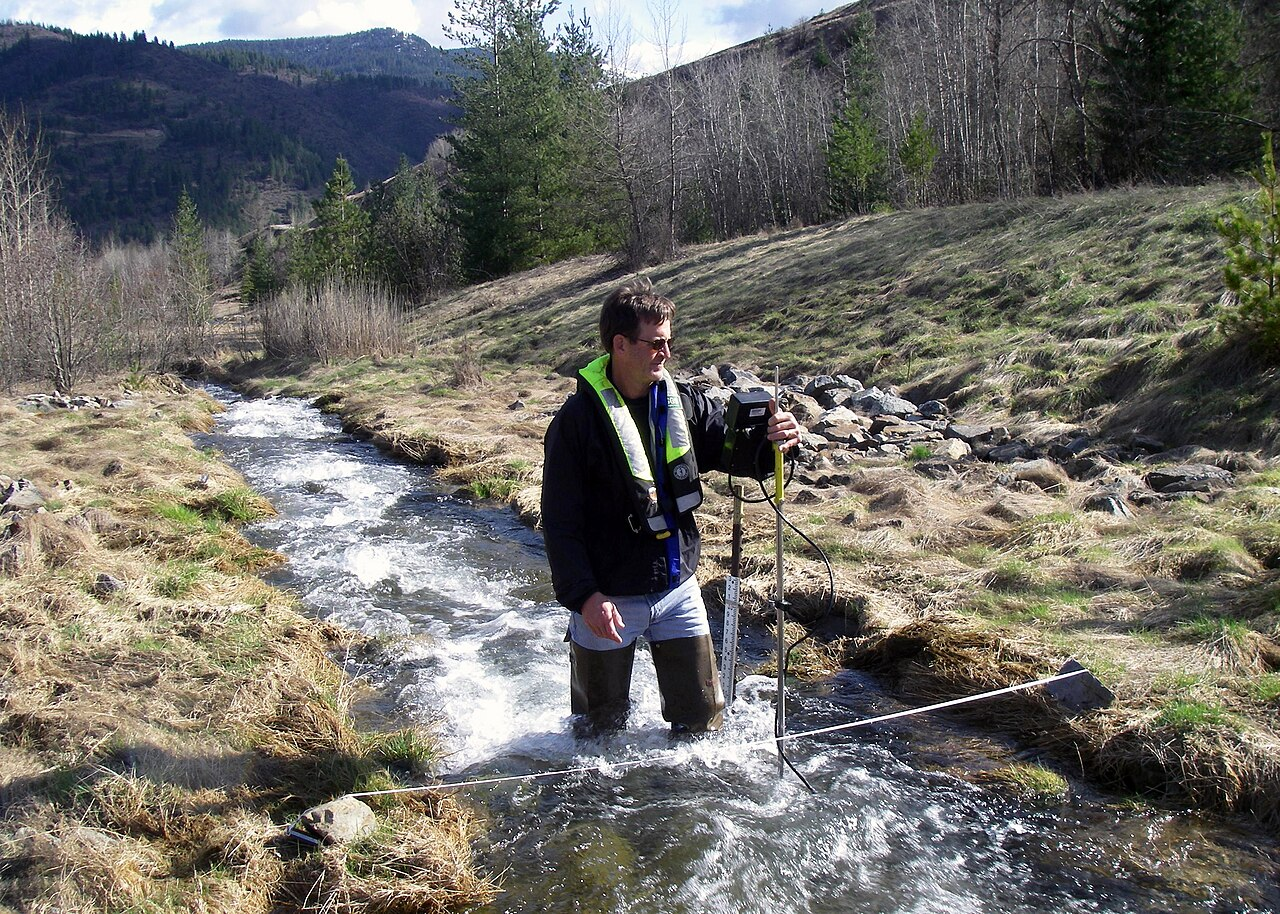
\includegraphics[height=4.6cm]{images/book2/g10-usgs-hydrologist-streamflow.jpg}\hspace{0.3cm}%
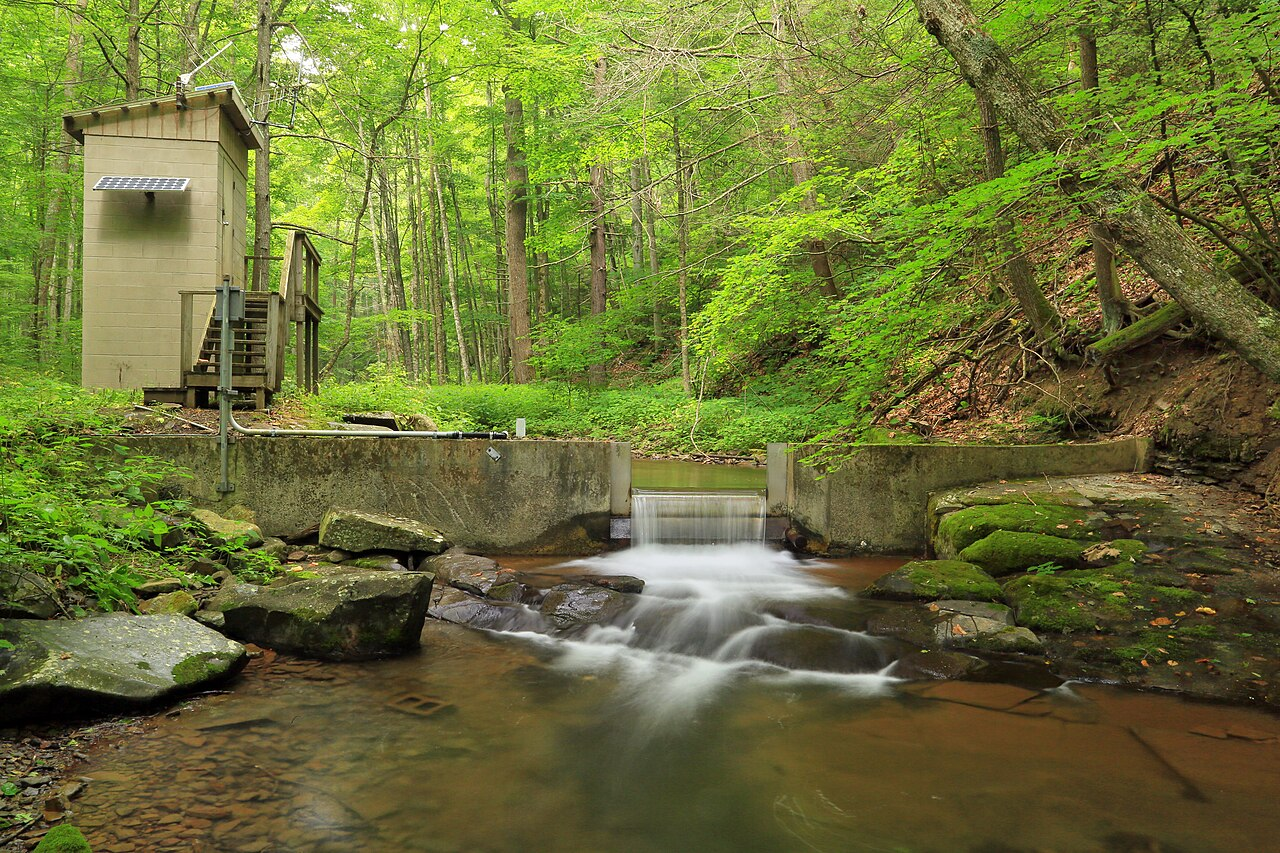
\includegraphics[height=4.6cm]{images/book2/g10-usgs-streamgage.jpg}

{\small 左图：水文学家用流速–面积法测量山间溪流的\omterm{def:g10:drainage-basins:discharge}{流量}；
横跨溪流拉紧的卷尺标出测垂线位置，测杆上挂着流速仪。
右图：林间溪流上的水文站，小屋内装有仪器，
用于记录小堰后的水位。
照片：美国地质调查局
（公有领域）。}
\end{omfigure}

实测\omterm{def:g10:drainage-basins:discharge}{流量}费时，无法连续进行。水文站则
不间断地记录水位。若干次在不同水位下的实测
结果给出水位与\omterm{def:g10:drainage-basins:discharge}{流量}的关系曲线，水文站据此将
所记录的每个水位换算为\omterm{def:g10:drainage-basins:discharge}{流量}。

大河的\omterm{def:g10:drainage-basins:discharge}{流量}十分惊人。1972 年至 2003 年间，亚马孙河平均
每秒向大西洋输送约 \qty{206000}{m^3/s} 的水，误差约在
\qty{6}{\percent} 以内，约占世界河流输入大海的全部淡水的
\qty{17}{\percent}。密西西比河平均每秒向
墨西哥湾输送 \num{593000} 立方英尺，约 \qty{16800}{m^3/s}，
亚马孙河的\omterm{def:g10:drainage-basins:discharge}{流量}约为其 12 倍。
% ledger: callede:amazon, kammerer:mississippi

\section{流量过程线}

\begin{definition}[流量过程线；基流；滞后时间]\label{def:g10:drainage-basins:hydrograph}
河流某一点的\omterm{def:g10:drainage-basins:discharge}{流量}随时间变化的图像称为\emph{流量过程线}\index{流量过程线}。
\emph{基流}\index{基流}是由地下水补给的那部分\omterm{def:g10:drainage-basins:discharge}{流量}，
它使河流在降雨间隙仍能保持流动。
洪水的\emph{滞后时间}\index{滞后时间}是\omterm{def:g10:drainage-basins:drainage-basin}{流域}降雨峰值
与\omterm{def:g10:drainage-basins:discharge}{流量}峰值之间的时间间隔。
\end{definition}

\begin{omfigure}
\begin{tikzpicture}[x=1cm, y=1cm, font=\footnotesize]
  \draw[-{Stealth}] (0,0) -- (10.2,0) node[below left] {时间};
  \draw[-{Stealth}] (0,0) -- (0,5.9) node[above right] {流量};
  % rain bars hanging from the top
  \draw[black!50] (0,5.4) -- (10,5.4);
  \foreach \x/\h in {1.0/0.15, 1.3/0.35, 1.6/0.55, 1.9/0.4, 2.2/0.2} {
    \fill[omWxRain!70] (\x,5.4) rectangle ++(0.28,-\h);
  }
  \node[anchor=south west] at (2.6,5.4) {流域上的降雨};
  % baseflow and hydrograph
  \fill[omSea] (0,0.7) -- (2.0,0.7) .. controls (2.8,0.8) and (3.3,3.3) .. (4.0,3.6)
    .. controls (4.6,3.6) and (5.1,2.1) .. (6.0,1.55) .. controls (7.0,1.0) and (8.0,0.85) .. (10,0.8)
    -- (10,0) -- (0,0) -- cycle;
  \fill[omLithAlluv] (0,0) -- (0,0.7) -- (2.0,0.7) .. controls (3.5,0.68) and (5.5,0.75) .. (6.6,0.95)
    .. controls (8,1.0) and (9,0.85) .. (10,0.8) -- (10,0) -- cycle;
  \draw[omDef, line width=1.2pt] (0,0.7) -- (2.0,0.7) .. controls (2.8,0.8) and (3.3,3.3) .. (4.0,3.6)
    .. controls (4.6,3.6) and (5.1,2.1) .. (6.0,1.55) .. controls (7.0,1.0) and (8.0,0.85) .. (10,0.8);
  \draw[black!60, dashed] (2.0,0.7) .. controls (3.5,0.68) and (5.5,0.75) .. (6.6,0.95);
  % lag time
  \draw[black!60, densely dotted] (1.74,4.85) -- (1.74,4.3);
  \draw[black!60, densely dotted] (3.98,3.65) -- (3.98,4.3);
  \draw[{Stealth}-{Stealth}] (1.74,4.3) -- node[above] {滞后时间} (3.98,4.3);
  % labels
  \node[anchor=west] at (4.2,3.75) {峰值};
  \node[anchor=east, align=right] at (2.9,2.2) {涨水 \\段};
  \node[anchor=west, align=left] at (5.4,2.3) {退水段};
  \node[align=center] at (4.5,1.25) {径流};
  \node at (8.2,0.4) {基流};
\end{tikzpicture}

{\small 洪水的\omterm{def:g10:drainage-basins:hydrograph}{流量过程线}（示意图）。降雨之后，\omterm{def:g10:drainage-basins:discharge}{流量}
上升至峰值，然后回落得更为缓慢；曲线下方的面积即为
水量体积。由地下水补给的\omterm{def:g10:drainage-basins:hydrograph}{基流}变化不大；其余部分为
降雨迅速汇入河流的径流。}
\end{omfigure}

暴雨中的水到达河流的时间各不相同。靠近河道的降雨
几分钟或几小时内即可到达；远在上游的降雨需要
长得多的时间，因为水必须沿坡面流下，再沿河道流动。
因此\omterm{def:g10:drainage-basins:discharge}{流量}急剧上升，进入\emph{涨水段}，而附近坡地
的水先行到达，大部分水同时到达时形成峰值，随后
\omterm{def:g10:drainage-basins:discharge}{流量}较缓慢地下降，进入\emph{退水段}，最后的水从\omterm{def:g10:drainage-basins:drainage-basin}{流域}
远端和土壤中排出。\omterm{def:g10:drainage-basins:drainage-basin}{流域}越大，
\omterm{def:g10:drainage-basins:hydrograph}{滞后时间}越长：小溪为数小时，大河则为数天。

有些\omterm{def:g10:drainage-basins:drainage-basin}{流域}形成\emph{陡涨型}洪水，峰值高而突然，\omterm{def:g10:drainage-basins:hydrograph}{滞后时间}短；
另一些\omterm{def:g10:drainage-basins:drainage-basin}{流域}则形成缓慢、平缓的洪水。同样的降雨在以下情况下会
形成更为陡涨的洪水：
\begin{itemize}
  \item \omterm{def:g10:drainage-basins:drainage-basin}{流域}面积小、坡度陡，
        水流需要走的路径短且快；
  \item 地面很少能让水渗入：裸露的岩石、黏土、
        已经饱水的地面、冻结的地面，尤其是城镇的屋顶、道路
        和停车场，它们几乎把全部降雨直接送入排水管
        和溪流；
  \item \omterm{def:g10:drainage-basins:drainage-basin}{流域}内溪流与排水网络密集，
        能迅速汇集水流。
\end{itemize}
森林、深厚的透水土壤和宽阔的河漫滩则相反：它们截留水分，
使水缓慢释放，从而降低并延缓洪峰。

\subsection*{一次真实的洪水}

美国东部的波托马克河在华盛顿附近一个水文站以上
的汇水\omterm{def:g10:drainage-basins:drainage-basin}{流域}面积为 \num{11560} 平方英里，约 \qty{29900}{km^2}。
1996 年 1 月，该水文站记录了
如下图所示的\omterm{def:g10:drainage-basins:hydrograph}{流量过程线}。
% ledger: data:b2-usgs-potomac

\begin{omfigure}
\begin{tikzpicture}
\begin{axis}[omrecord, width=0.86\linewidth, height=6cm, xmin=0, xmax=55, ymin=0, ymax=10000,
  xtick={0,10,20,30,40,50}, xticklabels={1月5日, 1月15日, 1月25日, 2月4日, 2月14日, 2月24日},
  ylabel={流量 (\unit{m^3/s})}, xlabel={1996},
  tick label style={font=\small}, label style={font=\small},
  scaled y ticks=false, yticklabel style={/pgf/number format/fixed}]
\addplot[omDef, line width=1.1pt, mark=*, mark size=1.1pt] table[x=day, y=q] {figdata/out/grade-10-flood_frequency-hydrograph.dat};
\node[anchor=west, font=\footnotesize] at (axis cs:17,9231) {\qty{9231}{m^3/s}（1月21日）};
\draw[black!60, dashed] (axis cs:5,334) -- (axis cs:13,334);
\node[anchor=south, font=\footnotesize] at (axis cs:9,1000) {约 \qty{330}{m^3/s}};
\draw[black!60] (axis cs:9,1000) -- (axis cs:9,390);
\end{axis}
\end{tikzpicture}

{\small 华盛顿附近波托马克河的日平均\omterm{def:g10:drainage-basins:discharge}{流量}，时段为
1996年1月5日至2月29日。洪水于1月18日由\qty{362}{m^3/s}涨起，
三天后超过\qty{9000}{m^3/s}，随后数周回落，
1月底又有一次较小的涨水。数据：美国地质调查局，
站点 01646500。}
\end{omfigure}
% values computed in figdata/grade-10/flood_frequency.py (hydro_peak_m3s 9231, hydro_before_mean 334)

洪水来临前的几天，河流\omterm{def:g10:drainage-basins:discharge}{流量}约为\qty{330}{m^3/s}，即其
\omterm{def:g10:drainage-basins:hydrograph}{基流}。1月21日日平均\omterm{def:g10:drainage-basins:discharge}{流量}达到\qty{9231}{m^3/s}，几乎
为\omterm{def:g10:drainage-basins:hydrograph}{基流}的三十倍。把当日经过测站的水
平铺于整个\omterm{def:g10:drainage-basins:drainage-basin}{流域}，将形成一层
$9231 \times 86400 / (29\,900 \times 10^6) \approx \qty{0.027}{m}$，约
\qty{27}{mm}深：一场大暴雨，在一天之内
从整个\omterm{def:g10:drainage-basins:drainage-basin}{流域}同时汇入。
% ledger: data:b2-usgs-potomac (hydro_peak_mm_per_day 26.6 in figdata/grade-10/flood_frequency.py)

\section{洪水与重现期}

一座城镇应当预期多大的洪水？答案来自过去：
运行数十年的水文测站，记录下每年的最大\omterm{def:g10:drainage-basins:discharge}{流量}，
即\emph{年最大洪峰}。小洪峰几乎年年都有，
大洪峰则很少出现。洪水越罕见，其规模越大。

\begin{definition}[重现期]\label{def:g10:drainage-basins:return-period}
洪水的\emph{重现期}\index{重现期} $T$ 是指
年最大洪峰等于或超过该值的各年之间的平均间隔（以年计）。
重现期为 $T$ 的洪水，即\emph{$T$ 年一遇洪水}，其在任一年中
被达到或超过的概率为 $1/T$。
\end{definition}

百年一遇洪水并非像时刻表那样每一百年来一次，
而是指每年都有百分之一的机会被达到或超过的洪水，
每年如此，与前一年发生什么无关。两次洪水可以
连续出现在相邻两年；一个世纪也可能一次都没有。

\begin{method}[由年最大洪峰记录求重现期]\label{met:g10:drainage-basins:return-periods}
\begin{enumerate}
  \item 列出 $n$ 年的年最大洪峰。
  \item 将其从大到小排列（最大者秩 $m = 1$，
        最小者秩 $m = n$）。
  \item 秩为 $m$ 的洪峰，其\omterm{def:g10:drainage-basins:return-period}{重现期}取 $T = (n + 1)/m$。
  \item 将洪峰对 $T$ 作图，横轴取 $T$ 的对数刻度，并
        读出所需\omterm{def:g10:drainage-basins:return-period}{重现期}对应的\omterm{def:g10:drainage-basins:discharge}{流量}。
\end{enumerate}
\end{method}

因此，$n$ 个洪峰中最大者的\omterm{def:g10:drainage-basins:return-period}{重现期}为 $T = n + 1$ 年：在一份
\num{95}~年的记录中即为 \num{96}~年。该公式反映的是记录所显示的事实：
秩为 $m$ 的洪峰，被达到或超过的年数为 $m$，
在 $n$ 年之中约每 $n/m$ 年一次。该方法无法可靠地外推到超过
记录长度之外：仅有 \num{50}~年的记录，难以说明
\num{1000}~年一遇洪水。

\begin{omfigure}
\begin{tikzpicture}
\begin{axis}[omrecord, width=0.86\linewidth, height=6.2cm, xmode=log, xmin=0.9, xmax=150,
  ymin=0, ymax=15000, xlabel={重现期 $T$（年）}, ylabel={年最大洪峰（\unit{m^3/s}）},
  xtick={1,2,5,10,20,50,100}, xticklabels={1,2,5,10,20,50,100},
  tick label style={font=\small}, label style={font=\small},
  scaled y ticks=false, yticklabel style={/pgf/number format/fixed}]
\addplot[only marks, mark=*, mark size=1.5pt, omDef] table[x=T, y=peak] {figdata/out/grade-10-flood_frequency-ranked.dat};
\node[anchor=east, font=\footnotesize] at (axis cs:92,13705) {1936};
\node[anchor=east, font=\footnotesize] at (axis cs:46,12658) {1942};
\node[anchor=south, font=\footnotesize] at (axis cs:32,10300) {1972};
\node[anchor=north west, font=\footnotesize, align=left] at (axis cs:1.1,14000) {华盛顿附近的波托马克河，\\1931--2025 年各年最大洪峰（$n = 95$）};
\end{axis}
\end{tikzpicture}

{\small 华盛顿附近波托马克河的\num{95}个年最大洪峰，按大小排序，
并与其\omterm{def:g10:drainage-basins:return-period}{重现期} $T = (n+1)/m$ 作图。最大者出现于
1936年3月，其\omterm{def:g10:drainage-basins:return-period}{重现期}为 $T = 96$ 年。数据：美国地质调查局，站点 01646500。}
\end{omfigure}
% values computed in figdata/grade-10/flood_frequency.py

\begin{dated}{2026}
在华盛顿附近波托马克河1931年至2025年的记录中，
最大的五次年最大洪峰分别出现于1936年3月（\qty{13700}{m^3/s}）、1942年10月、
1972年6月、1937年4月和1996年1月，其中最后两者
相等，均为\qty{9830}{m^3/s}。
% ledger: data:b2-usgs-potomac
\end{dated}

\subsection*{多年间洪水发生的概率}

房屋或桥梁可使用数十年。对它们而言，要紧的不是
某一年发生洪水的概率，而是整个使用期内的概率。

\begin{proposition}[$N$ 年中至少发生一次洪水]\label{prop:g10:drainage-basins:chance}
若各年相互独立，则\omterm{def:g10:drainage-basins:return-period}{重现期}为
$T$ 的洪水在 $N$ 年中至少被达到或超过一次的概率为
\[
P = 1 - \left(1 - \frac{1}{T}\right)^{N}.
\]
\end{proposition}

\begin{proof}
在某一年中，洪水\emph{不}发生的概率为
$1 - 1/T$。各年相互独立，洪水在
$N$ 年中均不发生的概率，等于 $N$ 个此类因子之积 $(1 - 1/T)^N$。
“至少一次”这一事件的对立事件为“从不”，因此其概率为
$1 - (1 - 1/T)^N$。
\end{proof}

对于百年一遇洪水，在三十年内，$(0.99)^{30} \approx 0.740$，因此
$P \approx 0.26$，即四分之一的机会。在一百年内，$(0.99)^{100}
\approx 0.366$，$P \approx 0.63$：百年一遇洪水
远非必然在一百年内到来。

\begin{omfigure}
\begin{tikzpicture}
\begin{axis}[omrecord, width=0.82\linewidth, height=5.8cm, xmin=0, xmax=100, ymin=0, ymax=1,
  xlabel={年数 $N$}, ylabel={至少发生一次洪水的概率},
  ytick={0,0.2,0.4,0.6,0.8,1}, yticklabels={0, 20\,\%, 40\,\%, 60\,\%, 80\,\%, 100\,\%},
  tick label style={font=\small}, label style={font=\small},
  legend pos=south east, legend style={font=\footnotesize}]
\addplot[omThm, line width=1pt] table[x=n, y=p10] {figdata/out/grade-10-flood_frequency-chance.dat};
\addplot[omProp, line width=1pt] table[x=n, y=p50] {figdata/out/grade-10-flood_frequency-chance.dat};
\addplot[omDef, line width=1pt] table[x=n, y=p100] {figdata/out/grade-10-flood_frequency-chance.dat};
\legend{{10年一遇洪水}, {50年一遇洪水}, {100年一遇洪水}}
\draw[black!60, dashed] (axis cs:30,0) -- (axis cs:30,0.2603) -- (axis cs:0,0.2603);
\fill[omDef] (axis cs:30,0.2603) circle (2pt);
\node[anchor=north west, font=\footnotesize] at (axis cs:31,0.22) {30年内 26\,\%};
\end{axis}
\end{tikzpicture}

{\small \omterm{def:g10:drainage-basins:return-period}{重现期}为 10、50 或 100 年的洪水在 $N$ 年内
至少发生一次的概率。}
\end{omfigure}
% values computed in figdata/grade-10/flood_frequency.py (chance_100_30 0.2603)

\section{水坝与堤防}

人类很早就修建了改变洪水流经方式的建筑物。其中两类建筑的作用
方式恰好相反。

\emph{水坝}拦起一个储库。洪水到来时，部分洪水蓄入储库，
使库水位上升，之后再在较长时间内泄放。
坝下游通过的水量相同，但水流被分散：洪峰
更低、出现更晚。只要库中仍有余量，储库便能削减洪水；
库满之后，流入的水全部继续下泄。

\emph{堤防}是沿河修筑的土埂，用以阻挡洪水漫入
河漫滩。两堤之间，水无法铺展；要以相同的\omterm{def:g10:drainage-basins:discharge}{流量}通过较窄的
断面，水位就必须抬高，流速也必须加快。
只要堤防坚固、未被洪水漫顶，堤后的土地便保持干燥。
但在洪水期间，河漫滩不再蓄水，
因此更多、更早的水流向下游。

\begin{omfigure}
\begin{tikzpicture}[x=0.62cm, y=0.62cm, font=\footnotesize]
  \begin{scope}
    \draw[-{Stealth}] (0,0) -- (9.4,0) node[below left] {时间};
    \draw[-{Stealth}] (0,0) -- (0,6.0) node[above right] {流量};
    \draw[omDef, line width=1.2pt] (0,0.6) -- (1,0.6) .. controls (1.8,0.7) and (2.2,5.2) .. (2.8,5.2)
      .. controls (3.5,5.2) and (4,1.6) .. (5,1.0) .. controls (6,0.7) and (7.5,0.6) .. (9,0.6);
    \draw[omThm, line width=1.2pt, dashed] (0,0.6) -- (1.3,0.6) .. controls (2.3,0.75) and (3.0,3.3) .. (3.8,3.3)
      .. controls (4.7,3.3) and (5.8,1.5) .. (6.8,1.0) .. controls (7.6,0.75) and (8.3,0.65) .. (9,0.6);
    \node[anchor=west, text=omDef] at (3.0,5.35) {流入储库};
    \node[anchor=west, text=omThm] at (4.2,3.55) {坝下};
    \node[anchor=north] at (4.5,-0.45) {(a) 水坝：洪峰更低、更晚};
  \end{scope}
  \begin{scope}[xshift=7.2cm]
    \fill[omLithAlluv] (0,0) -- (10,0) -- (10,1.8) -- (0,1.8) -- cycle;
    \fill[white] (3.5,1.8) -- (3.9,0.4) -- (6.1,0.4) -- (6.5,1.8) -- cycle;
    \fill[omSea] (0.4,2.3) -- (3.25,2.3) -- (3.5,1.8) -- (3.9,0.4) -- (6.1,0.4) -- (6.5,1.8) -- (6.75,2.3) -- (9.6,2.3) -- (9.6,1.8) -- (0.4,1.8) -- cycle;
    \draw[line width=0.8pt, brown!60!black] (0,1.8) -- (3.5,1.8) -- (3.9,0.4) -- (6.1,0.4) -- (6.5,1.8) -- (10,1.8);
    \draw[omDef!70!black] (0.4,2.3) -- (9.6,2.3);
    \node[anchor=south, text=omDef!70!black, align=center] at (1.5,2.35) {无 \\堤防};
    % levees
    \fill[brown!45] (2.6,1.8) -- (3.0,3.9) -- (3.3,3.9) -- (3.5,1.8) -- cycle;
    \fill[brown!45] (6.5,1.8) -- (6.7,3.9) -- (7.0,3.9) -- (7.4,1.8) -- cycle;
    \fill[omSea!70!omDef] (3.5,1.8) -- (3.9,0.4) -- (6.1,0.4) -- (6.5,1.8) -- (6.65,3.4) -- (3.35,3.4) -- cycle;
    \draw[omThm, line width=0.8pt, dashed] (3.35,3.4) -- (6.65,3.4);
    \node[anchor=south, text=omThm] at (5,3.95) {有堤防};
    \draw[omThm] (5,3.95) -- (5,3.45);
    \node[anchor=north] at (5,-0.45) {(b) 堤防：洪水水位更高};
  \end{scope}
\end{tikzpicture}

{\small 示意图。(a) 储库蓄存部分洪水，并在之后泄放：
坝下的洪峰更低、出现更晚。(b) 无堤防时，洪水在河漫滩上薄薄地铺展；
有堤防时，同样的\omterm{def:g10:drainage-basins:discharge}{流量}须从两堤之间的狭窄断面通过，
因而水位高得多。}
\end{omfigure}

\section{练习}

\begin{exercise}[$\star$]\label{exo:g10:drainage-basins:1}
定义\omterm{def:g10:drainage-basins:drainage-basin}{流域}和\omterm{def:g10:drainage-basins:drainage-basin}{分水岭}。相距一米落下的两滴雨滴，
为什么会分别汇入两个不同的海？
\end{exercise}

\begin{exercise}[$\star$]\label{exo:g10:drainage-basins:2}
定义河流的\omterm{def:g10:drainage-basins:discharge}{流量}并给出其单位。一天内有多少升水
通过一条\omterm{def:g10:drainage-basins:discharge}{流量}为 \qty{1}{m^3/s} 的河流上的某一点？
\end{exercise}

\begin{exercise}[$\star$]\label{exo:g10:drainage-basins:3}
根据 1996 年 1 月波托马克河的\omterm{def:g10:drainage-basins:hydrograph}{流量过程线}，读出
洪水前的\omterm{def:g10:drainage-basins:hydrograph}{基流}、洪峰\omterm{def:g10:drainage-basins:discharge}{流量}及其出现日期，以及涨水过程
所用的天数。
\end{exercise}

\begin{exercise}[$\star$]\label{exo:g10:drainage-basins:4}
求 \num{50} 年一遇的洪水在下一年
被达到或超过的概率。去年发生了一次
\num{50} 年一遇的洪水，今年发生的可能性是否更小？
\end{exercise}

\begin{exercise}[$\star$]\label{exo:g10:drainage-basins:5}
密西西比河平均每秒向大海输送 \num{593000} 立方英尺
的水（\num{1}~英尺 = \qty{0.3048}{m}）。将此\omterm{def:g10:drainage-basins:discharge}{流量}换算为
\unit{m^3/s}，并与亚马孙河的
\qty{206000}{m^3/s} 相比较。
\end{exercise}

\begin{exercise}[$\star\star$]\label{exo:g10:drainage-basins:6}
一位水文学家用四条测深垂线测量一条溪流，相邻垂线相距 \qty{1.5}{m}。
各测深垂线处的深度依次为 \num{0.3}、\num{0.6}、\num{0.7} 和 \qty{0.4}{m}；
平均流速依次为 \num{0.2}、\num{0.5}、\num{0.6} 和 \qty{0.3}{m/s}。
求过水截面面积、\omterm{def:g10:drainage-basins:discharge}{流量}及平均流速。
\end{exercise}

\begin{exercise}[$\star\star$]\label{exo:g10:drainage-basins:7}
一场风暴使瓦尔登河的整个\omterm{def:g10:drainage-basins:drainage-basin}{流域}降下 \qty{20}{mm} 的雨量，
图上所示\omterm{def:g10:drainage-basins:drainage-basin}{流域}面积为 \qty{66}{km^2}。这些雨水的体积是多少？若其全部
在两天内汇至出口，则平均额外\omterm{def:g10:drainage-basins:discharge}{流量}为多少？
\end{exercise}

\begin{exercise}[$\star\star$]\label{exo:g10:drainage-basins:8}
一条小河九年间每年的洪峰\omterm{def:g10:drainage-basins:discharge}{流量}依次为（单位：\unit{m^3/s}）：
\num{42}、\num{65}、\num{38}、\num{120}、\num{51}、\num{47}、\num{88}，
\num{35}、\num{59}。将这些洪峰排序，并求三个最大洪峰的
\omterm{def:g10:drainage-basins:return-period}{重现期}。中位数对应的洪峰的\omterm{def:g10:drainage-basins:return-period}{重现期}是多少？
\end{exercise}

\begin{exercise}[$\star\star$]\label{exo:g10:drainage-basins:9}
同一场风暴落在两个面积相同的\omterm{def:g10:drainage-basins:drainage-basin}{流域}上：一个陡峭，
且被城镇覆盖；另一个坡度平缓，有森林覆盖。
在同一坐标系中画出两者的水文过程线示意图，并解释其差异。
\end{exercise}

\begin{exercise}[$\star\star$]\label{exo:g10:drainage-basins:10}
1996 年 1 月 21 日洪峰时，波托马克河输出的\omterm{def:g10:drainage-basins:discharge}{流量}为 \qty{9231}{m^3/s}，
\omterm{def:g10:drainage-basins:drainage-basin}{流域}面积为 \qty{29900}{km^2}。这一天的\omterm{def:g10:drainage-basins:discharge}{流量}若均匀分布于整个\omterm{def:g10:drainage-basins:drainage-basin}{流域}，
相当于多深的水层？并与\omterm{def:g10:drainage-basins:hydrograph}{基流}相比较。
\omterm{def:g10:drainage-basins:hydrograph}{基流}为 \qty{330}{m^3/s}。
\end{exercise}

\begin{exercise}[$\star\star$]\label{exo:g10:drainage-basins:11}
求 \num{10} 年一遇的洪水在 \num{10} 年内至少出现一次的概率；
以及这十年内完全不出现的概率。
\end{exercise}

\begin{exercise}[$\star\star\star$]\label{exo:g10:drainage-basins:12}
洪水进入水库的\omterm{def:g10:drainage-basins:discharge}{流量}匀速上升，
一天内由 \qty{0}{m^3/s} 增至 \qty{1200}{m^3/s}，随后
两天内匀速降回 \qty{0}{m^3/s}（忽略\omterm{def:g10:drainage-basins:hydrograph}{基流}）。这次洪水带来的水量为多少？
大坝至多泄出 \qty{800}{m^3/s}，水库的蓄水容量为
6000 万 \unit{m^3}。它能否蓄住超过
\qty{800}{m^3/s} 的全部水量？
\end{exercise}

\begin{exercise}[$\star\star\star$]\label{exo:g10:drainage-basins:13}
一条宽 \qty{100}{m} 的河流在\omterm{def:g10:drainage-basins:discharge}{流量}为 \qty{800}{m^3/s} 时正好满岸，
流速为 \qty{2}{m/s}。此时来了一次\omterm{def:g10:drainage-basins:discharge}{流量}为 \qty{1200}{m^3/s} 的洪水。
\begin{enumerate}
  \item 若无堤防，多出的 \qty{400}{m^3/s} \omterm{def:g10:drainage-basins:discharge}{流量}将漫布于河漫滩上，
        河漫滩宽 \qty{900}{m}，流速为 \qty{0.5}{m/s}，
        河漫滩上的水有多深？
  \item 若有堤防，全部洪水均在堤间流过，流速为 \qty{2}{m/s}。
        河道水深为多少？水面高出河岸多少？
\end{enumerate}
\end{exercise}

\begin{exercise}[$\star\star\star$]\label{exo:g10:drainage-basins:14}
\omterm{def:g10:drainage-basins:return-period}{重现期} $T$ 取何值时，洪水
在 \num{30} 年内至少出现一次的机会为二分之一？
\end{exercise}

\begin{exercise}[$\star\star\star$]\label{exo:g10:drainage-basins:15}
将一张小地图划分为边长 \qty{100}{m} 的方格，各方格的高程（单位为米）如下（北在上方）。
水从某方格流向其四个相邻方格（北、南、东、西）中最低的一个，
前提是该相邻方格低于本方格；
位于 \qty{34}{m}（西北角）和 \qty{30}{m}（东南角）的方格
是两条溪流的出口。
\begin{center}
\begin{tabular}{|c|c|c|c|}
\hline
34 & 38 & 46 & 50 \\ \hline
37 & 42 & 48 & 47 \\ \hline
45 & 49 & 44 & 39 \\ \hline
51 & 46 & 37 & 30 \\ \hline
\end{tabular}
\end{center}
画出每个方格的水流方向，求出每个出口的\omterm{def:g10:drainage-basins:drainage-basin}{流域}
及其面积，并画出\omterm{def:g10:drainage-basins:drainage-basin}{分水岭}。
\end{exercise}

\section{问题：百年一遇的洪水}

\begin{problem}[{周末问题——这条河多久会流入城镇？}]
\label{pb:g10:drainage-basins:1}
% ledger: data:b2-usgs-potomac (values computed in figdata/grade-10/flood_frequency.py)
设想一座城镇位于波托马克河上，恰在华盛顿上游，
靠近一个每年记录该河最大\omterm{def:g10:drainage-basins:discharge}{流量}的水文站，
该站自 \num{1931} 年起逐年记录。下面给出各年的年洪峰\omterm{def:g10:drainage-basins:discharge}{流量}，
并附有本章给出的 1996 年 1 月水文过程线。

\begin{center}
\begin{tikzpicture}
\begin{axis}[omrecord, width=0.9\linewidth, height=5.4cm, ybar, bar width=1.6pt, xmin=1929, xmax=2027,
  ymin=0, ymax=15000, ylabel={年洪峰流量 (\unit{m^3/s})}, xlabel={年份},
  xtick={1930,1950,1970,1990,2010}, xticklabel style={/pgf/number format/1000 sep={}},
  tick label style={font=\small}, label style={font=\small},
  scaled y ticks=false, yticklabel style={/pgf/number format/fixed}]
\addplot[fill=omDef!70, draw=none] table[x=year, y=peak] {figdata/out/grade-10-flood_frequency-record.dat};
\draw[omThm, dashed] (axis cs:1929,9500) -- (axis cs:2027,9500);
\node[anchor=south east, font=\footnotesize, text=omThm] at (axis cs:2026,9500) {\qty{9500}{m^3/s}};
\end{axis}
\end{tikzpicture}

{\small 华盛顿附近波托马克河的年洪峰\omterm{def:g10:drainage-basins:discharge}{流量}，
水文年 1931--2025 年（水文年自 10 月至次年 9 月：1942 年 10 月的洪水计入 1943 年）。
数据来源：美国地质调查局，站点 01646500。}
\end{center}

\medskip
\noindent\textbf{第一部分——\omterm{def:g10:drainage-basins:drainage-basin}{流域}与\omterm{def:g10:drainage-basins:discharge}{流量}。}
\begin{enumerate}
  \item 该水文站的\omterm{def:g10:drainage-basins:drainage-basin}{流域}面积为 \num{11560} 平方英里
        （\num{1}~英里 = \qty{1.609}{km}）。将此面积换算为
        \unit{km^2}。
  \item 地图上哪条线界定了这一区域？
  \item 1936 年 3 月 19 日出现最大洪峰，其\omterm{def:g10:drainage-basins:discharge}{流量}为每秒 \num{484000} 立方英尺。
        将其换算为 \unit{m^3/s}（\num{1}~英尺 = 
        \qty{0.3048}{m}）。
  \item 年洪峰的中位数为 \qty{3341}{m^3/s}。
        1936 年的洪水是中位数的多少倍？
  \item 假设在 1936 年洪峰时，该河在水文站处平均宽 \qty{400}{m}，
        平均深 \qty{8}{m}。
        试求当时的平均流速。
\end{enumerate}

\medskip
\noindent\textbf{第二部分——读解 1996 年的洪水。}
\begin{enumerate}[resume]
  \item 在 1996 年 1 月的水文过程线上，
        洪水来临前几天的\omterm{def:g10:drainage-basins:hydrograph}{基流}是多少？
  \item 日\omterm{def:g10:drainage-basins:discharge}{流量}峰值是多少？出现在哪一天？
  \item 自 1 月 18 日的 \qty{362}{m^3/s} 起，
        涨至峰值共用了几天？
  \item 峰值当日经水文站流过的水量，
        若均匀分布于整个\omterm{def:g10:drainage-basins:drainage-basin}{流域}，相当于多深的水层？
  \item 1 月 29 日又出现一次较小的涨水，
        这对到达\omterm{def:g10:drainage-basins:drainage-basin}{流域}的水量说明了什么？
  \item 2 月 7 日\omterm{def:g10:drainage-basins:discharge}{流量}回落至 \qty{410}{m^3/s} 左右，
        这距峰值过去了多久？
        为什么退水段比涨水段持续得更久？
\end{enumerate}

\medskip
\noindent\textbf{第三部分——洪水排序。}
\begin{enumerate}[resume]
  \item 记录中共有 $n = 95$ 个年最大洪峰，
        该方法赋予最大一次洪水的\omterm{def:g10:drainage-basins:return-period}{重现期}是多少？
  \item 1942 年 10 月的洪峰（\qty{12658}{m^3/s}）排名第二，
        其\omterm{def:g10:drainage-basins:return-period}{重现期}是多少？
  \item 1972 年 6 月的洪峰（\qty{10166}{m^3/s}）排名第三，
        其\omterm{def:g10:drainage-basins:return-period}{重现期}是多少？
  \item 1937 年 4 月与 1996 年 1 月的两次洪水\omterm{def:g10:drainage-basins:discharge}{流量}相等（\qty{9826}{m^3/s}），
        若二者分别排第 4 位和第 5 位，它们各得到怎样的\omterm{def:g10:drainage-basins:return-period}{重现期}？
        并列取值对这里的结果影响大吗？
  \item 根据柱状图，数一数洪峰超过 \qty{9500}{m^3/s} 的年份，
        估算任一年出现此类洪峰的概率，
        并求其\omterm{def:g10:drainage-basins:return-period}{重现期}。
\end{enumerate}

\medskip
\noindent\textbf{第四部分——洪水发生的概率。}
\begin{enumerate}[resume]
  \item \num{100} 年一遇洪水在某一年中被达到或
        超过的概率是多少？
  \item 在该年份中，该洪水未被达到或超过的概率是多少？
  \item 该洪水在 \num{30} 年内均不出现的概率是多少，
        这段时间约是一个家庭在河边住房中可能居住的时长？
  \item \num{30} 年内至少出现一次 \num{100} 年一遇洪水的
        机会是多少？
\end{enumerate}
\end{problem}
